\documentclass[12pt,a4paper]{article}
\usepackage[utf8]{inputenc} %accents
\usepackage{tikz}

\usetikzlibrary{decorations.pathreplacing,shapes,arrows,positioning,backgrounds}
\usetikzlibrary{calc,automata,petri,positioning,calc} 
%\usetikzlibrary{graphdrawing.trees}
\usetikzlibrary{patterns}
\usepackage{textcomp}
\usepackage[T1]{fontenc}%accents jolis
%\usepackage{lxfonts}

%\usepackage[round,numbers]{natbib}
\usepackage[french]{babel} %règles orthographes  
\usepackage{amsmath}
\usepackage{esint}
\usepackage{datetime}

\usepackage{amssymb}
\usepackage{mathtools}
\usepackage{subcaption,float}

%\usepackage[a4paper,left=1cm,right=2cm,top=2cm,bottom=1.5cm]{geometry}
\usepackage[margin=2cm]{geometry}
\graphicspath{{C:/Users/Qlala/Documents/M2_SETI/modele/}}

\usepackage{pdfpages}
\usepackage{comment}
\usepackage{libertine}
\usepackage{graphicx,eso-pic}
\usepackage{pythontex}
\usepackage{minted}
\usepackage{longtable}
\usepackage{latexsym}
\usepackage{svg}
\usepackage[outline]{contour}
\usepackage{pgfplots}
\usepackage{sectsty}

\usepgfplotslibrary{external} 

%\tikzexternalize[prefix=tikz/]



\usepackage{geometry}



\setpygmentsfv{xleftmargin=4ex} %Pass fancyvrb options, in this case, left margin
\usepackage{multirow}
\usepackage{listings}
\usepackage{schemabloc}
\usepackage[space]{grffile}
\usepackage{array}
\usepackage{xcolor}
\usepackage{color}
\definecolor{gray}{rgb}{0.4,0.4,0.4}
\definecolor{darkblue}{rgb}{0.0,0.0,0.6}
\definecolor{cyan}{rgb}{0.0,0.6,0.6}
\usepackage{colortbl}
\usepackage{hhline}
\usepackage{listingsutf8}
\usepackage{siunitx}

%hyper link
%\addbibresource{TER_biblio.bib}
\usepackage[colorlinks,allcolors=black]{hyperref}
\usepackage{url}
\hypersetup{urlcolor=blue}

\usepackage[french,onelanguage]{algorithm2e}

\setlength{\parindent}{0cm}
\setlength{\parskip}{1ex plus 0.5ex minus 0.2ex}
\newcommand{\hsp}{\hspace{20pt}}
\newcommand{\HRule}{\rule{\linewidth}{0.5mm}}
\newcommand{\z}{z^{-1}}
\usepackage{multicol}
\lstset{inputencoding=latin1}
\lstset{language=Matlab}

\newcommand{\complex}{\mathbb{C}}
\newcommand{\N}{\mathbb{N}}
\newcommand{\real}{\mathbb{R}}%outil mathématique
\newcommand{\Z}{\mathbb{Z}}%outil mathématique
\newcommand{\LL}{\mathbb{L}}%outil mathématique
\newcommand{\CodeC}[1]{%
\begin[language=C++]{lstlisting} ^^J
#1 ^^J
\end{lstlisting}
}
\DeclarePairedDelimiter{\norm}{\lVert}{\rVert}
\DeclarePairedDelimiter{\abs}{\lvert}{\rvert}

\makeatletter
\let\oldabs\abs
\def\abs{\@ifstar{\oldabs}{\oldabs*}}
%
%\let\oldnorm\norm
%\def\norm{\@ifstar{\oldnorm}{\oldnorm*}}
\makeatother
\newenvironment{static_figure}
    {\begin{center}
%\newgeometry{top=3cm,left=0cm,right=0cm,bottom=3cm,}
%     \setlength{\leftskip}{-1.5cm}
%     \setlength{\rightskip}{-1.5cm}
     \center
          
    \begin{minipage}[c]{\linewidth}
    
 \begin{center}
 
}{
 \end{center}
 \end{minipage}
 \end{center} 
 }
\usepackage{color}

\usepackage[edges]{forest}

\definecolor{folderbg}{RGB}{124,166,198}
\definecolor{folderborder}{RGB}{110,144,169}
\newlength\Size
\setlength\Size{4pt}


\definecolor{folderbg}{RGB}{124,166,198}
\definecolor{folderborder}{RGB}{110,144,169}
\tikzset{%
  folder/.pic={%
    \filldraw [draw=folderborder, top color=folderbg!50, bottom color=folderbg] (-1.05*\Size,0.2\Size+5pt) rectangle ++(.75*\Size,-0.2\Size-5pt);
    \filldraw [draw=folderborder, top color=folderbg!50, bottom color=folderbg] (-1.15*\Size,-\Size) rectangle (1.15*\Size,\Size);
  },
  file/.pic={%
    \filldraw [draw=folderborder, top color=folderbg!5, bottom color=folderbg!10] (-\Size,.4*\Size+5pt) coordinate (a) |- (\Size,-1.2*\Size) coordinate (b) -- ++(0,1.6*\Size) coordinate (c) -- ++(-5pt,5pt) coordinate (d) -- cycle (d) |- (c) ;
  },
  root/.pic={%                                                                     
 \node[yshift=3\Size,anchor=north] {\includegraphics[width=3\Size]{im/usb.png} };  
  },                                                                               
  sln/.pic={%                                                                      
 \node[yshift=3\Size,anchor=north] {\includegraphics[width=3\Size]{im/sln.png} };  
  },                                                                              
  pdf/.pic={%                                                                      
 \node[yshift=3\Size,anchor=north] {\includegraphics[width=3\Size]{im/pdf.png} };  
  },                                                                               
}
%----------------------------------------------------------------
%state diagram
%--------------------------------------------------
\tikzset{
    place/.style={
        circle,
        thick,
        draw=black,
        fill=gray!50,
        minimum size=6mm,
    },
        state/.style={
        circle,
        thick,
        draw=blue!75,
        fill=blue!20,
        minimum size=6mm,
    },
}

\forestset{%
  declare autowrapped toks={pic me}{},
  declare boolean register={pic root},
  pic root=0,
  pic dir tree/.style={%
    for tree={%
      folder,
      font=\ttfamily,
      grow'=0,
    },
    before typesetting nodes={%
      for tree={%
        edge label+/.option={pic me},
      },
      if pic root={
        tikz+={
          \pic at ([xshift=\Size].west) {root};
        },
        align={l}
      }{},
    },
  },
  pic me set/.code n args=2{%
    \forestset{%
      #1/.style={%
        inner xsep=2\Size,
        pic me={pic {#2}},
      }
    }
  },
  pic me set={directory}{folder},
  pic me set={file}{file},
  pic me set={sln}{sln},
  pic me set={pdf}{pdf},
}



\definecolor{mygreen}{rgb}{0,0.6,0}
\definecolor{mygray}{rgb}{0.5,0.5,0.5}
\definecolor{mymauve}{rgb}{0.58,0,0.82}
%style de node pour les tickpicture
\tikzstyle{decision} = [diamond, draw, fill=blue!20, 
     text badly centered, inner sep=0pt]
\tikzstyle{block} = [rectangle, draw, fill=blue!20, 
    text centered, rounded corners, minimum height=2em,align=center]
\tikzstyle{line} = [draw, -latex']
\tikzstyle{cloud} = [draw, ellipse,fill=red!20, node distance=3cm,
    minimum height=2em]
\tikzstyle{round} = [draw, circle,fill=red!20, node distance=3cm,
    minimum height=2em]
 %subsubsubsection
\setcounter{secnumdepth}{4}
\setcounter{tocdepth}{3}
\makeatletter
\newcounter {subsubsubsection}[subsubsection]
\renewcommand\thesubsubsubsection{\thesubsubsection .\@alph\c@subsubsubsection}
\newcommand\subsubsubsection{\@startsection{subsubsubsection}{4}{\z@}%
                                     {-3.25ex\@plus -1ex \@minus -.2ex}%
                                     {1.5ex \@plus .2ex}%
                                     {\normalfont\normalsize\bfseries}}
\newcommand*\l@subsubsubsection{\@dottedtocline{3}{10.0em}{4.1em}}
\newcommand*{\subsubsubsectionmark}[1]{}
\makeatother    
    
    
    \lstdefinelanguage{XML}
{
  morestring=[b]",
  morestring=[s]{>}{<},
  morecomment=[s]{<?}{?>},
  stringstyle=\color{black},
  identifierstyle=\color{darkblue},
  keywordstyle=\color{cyan},
  morekeywords={xmlns,version,type}% list your attributes here
}

\lstset{ %
  backgroundcolor=\color{white},   % choose the background color; you must add \usepackage{color} or \usepackage{xcolor}; should come as last argument
  basicstyle=\footnotesize,        % the size of the fonts that are used for the code
  breakatwhitespace=false,         % sets if automatic breaks should only happen at whitespace
  breaklines=true,                 % sets automatic line breaking
  captionpos=b,                    % sets the caption-position to bottom
  commentstyle=\color{mygreen},    % comment style
  deletekeywords={...},            % if you want to delete keywords from the given language
  escapeinside={\%*}{*)},          % if you want to add LaTeX within your code
  extendedchars=true,              % lets you use non-ASCII characters; for 8-bits encodings only, does not work with UTF-8
  frame=single,	                   % adds a frame around the code
  keepspaces=true,                 % keeps spaces in text, useful for keeping indentation of code (possibly needs columns=flexible)
  keywordstyle=\color{blue},       % keyword style
  language=Octave,                 % the language of the code
  morekeywords={*,...},            % if you want to add more keywords to the set
  numbers=left,                    % where to put the line-numbers; possible values are (none, left, right)
  numbersep=5pt,                   % how far the line-numbers are from the code
  numberstyle=\tiny\color{mygray}, % the style that is used for the line-numbers
  rulecolor=\color{black},         % if not set, the frame-color may be changed on line-breaks within not-black text (e.g. comments (green here))
  showspaces=false,                % show spaces everywhere adding particular underscores; it overrides 'showstringspaces'
  showstringspaces=false,          % underline spaces within strings only
  showtabs=false,                  % show tabs within strings adding particular underscores
  stepnumber=2,                    % the step between two line-numbers. If it's 1, each line will be numbered
  stringstyle=\color{mymauve},     % string literal style
  tabsize=2,	                   % sets default tabsize to 2 spaces
  title=\lstname,% show the filename of files included with \lstinputlisting; also try caption instead of title
  rangeprefix= ,% curly left brace plus space
  rangesuffix=% space plus curly right brace               
}

%\geometry{margin=1cm}
%\usepackage{scrlayer-scrpage}
%\cfoot[\pagemark]{\pagemark}   % odd   page, center position
\parindent=1cm 
%header
%\usepackage[notextcomp]{kpfonts}

\usepackage{fancyhdr}
%\pagestyle{fancy}
%\fancyhf{}

\usepackage[explicit]{titlesec}

%\renewcommand{\chaptermark}[1]{%
%  \markboth{%
%    \ifnum\value{chapter}>0
%      \thechapter.\space
%    \fi
%    #1%
%  }{}%
%}

%\newcommand\chapterimage[2][]{%
%%  \AddToShipoutPictureBG*{% Add picture to BackGround on this page only
%%    \AtTextLowerLeft{% Position at lower left of text block
%%      \hspace*{\textwidth}% Move over to upper right of text block
%%      \llap{% Ignore horizontal width and overlap to the left
%%        \smash{% Ignore vertical height
%%          \raisebox{-\height}{% Lower so top touches baseline
%%            \includegraphics[#1]{#2}}}}}}
%            
%\newpage            
            %}% Include image with options
%\usepackage[notextcomp]{kpfonts}

%\renewcommand{\headrulewidth}{2pt}
%\renewcommand{\footrulewidth}{1pt}
%\renewcommand{\chaptermark}[1]{\markboth{#1}{#1}}
%\renewcommand{\chaptermark}[1]{%
%\markboth{#1}{}}
%\titleformat{\chapter}{\bfseries\Large}{\arabic{chapter}.~}{0pt}{}
%\definecolor{darkblue}{rgb}{0.12,0.37,0.87}


%\titleformat{\chapter}
%  {\gdef\chapterlabel{}
%   \normalfont\sffamily\Huge\bfseries\scshape}
%  {\gdef\chapterlabel{\thechapter)\ }}{0pt}
  {%\chapterlabel#1
%  \begin{tikzpicture}[remember picture,overlay]
%    \node[yshift=-8cm] at (current page.north west)
%      {\begin{tikzpicture}[remember picture,overlay]
%        \draw[fill=black] (0,0) rectangle
%          (\paperwidth,4cm);
%\node[fill=black,rectangle,minimum width=\paperwidth,minimum height=8cm,anchor=south west,inner sep=0pt] at (0,0){\includegraphics[width=\paperwidth]{im/sc_chap.jpg}};
%        \node[anchor=east,xshift=.9\paperwidth,rectangle,
%              rounded corners=20pt,inner sep=11pt,
%              fill=darkblue,align=center,text=white,font=\LARGE]
%              {\chapterlabel#1};
%       \end{tikzpicture}
%      };
%   \end{tikzpicture}
%     \\[5cm]
%  %\newpage
%  }

%\titlespacing*{\chapter}{0pt}{50pt}{-60pt}
%\chapterfont{\color{darkblue}}  % sets colour of chapters
%\sectionfont{\color{darkblue}\bfseries}  % sets colour of sections
%\titleformat{\section}{\color{darkblue}\normalfont\fontsize{12}{17}\bfseries}{\thesection}{1em}{}



%\fancypagestyle{plain}{%chapter page
%  \fancyhf{}%
%\chead{\begin{tikzpicture}[remember picture,on background layer,overlay]
%    \node[yshift=0cm] at (current page.north east)
%      {\begin{tikzpicture}[remember picture,overlay]
%\node[fill=black,rectangle,minimum width=\paperwidth,minimum height=10cm,anchor=north east,inner %sep=0pt] at (0,0){\includegraphics[width=\paperwidth]{im/back.png}};
%       \end{tikzpicture}
%      };
%   \end{tikzpicture}}
%\cfoot{\raisebox{0.5cm}{\thepage}   }
%\rfoot{\raisebox{0.5cm}{\includegraphics[scale=0.5]{im/alstom.png}}}
%\lfoot{\includegraphics[scale=0.08]{im/EN.jpg}}
%\renewcommand{\headrulewidth}{2pt}
%\renewcommand{\footrulewidth}{1pt}
%}


%classical page
%\lhead{
%\begin{tikzpicture}[remember picture,on background layer,overlay]
%    \node[yshift=0cm] at (current page.north east)
%      {\begin{tikzpicture}[remember picture,overlay]
%\node[fill=black,rectangle,minimum width=\paperwidth,minimum height=10cm,anchor=north east,inner %sep=0pt] at (0,0){\includegraphics[width=\paperwidth]{im/back.png}};
%       \end{tikzpicture}
%      };
%   \end{tikzpicture}
%}

%\rhead{{ \small \MakeUppercase{\leftmark}}}
%\cfoot{\raisebox{0.5cm}{\thepage}   }
%\rfoot{\raisebox{0.5cm}{\includegraphics[scale=0.5]{im/alstom.png}}}
%\lfoot{\raisebox{0cm}{\includegraphics[scale=0.08]{im/EN.jpg}}}


%\def\extendedAppendix{1}
%\def\Presentation{0}



\begin{document}
\begin{titlepage}
\begin{center}
\vspace*{1cm}

\textbf{Master E3A}

\vspace{0.5cm}


Cours A2 : Systèmes Electroniques Embarqués

\vspace{1.5cm}
\mytitle

\vspace{1.5cm}
\theauthor

\vspace{1.5cm}
Encadré par :
\textbf{HAMMAMI Omar} et \textbf{LE PROVOST Hervé}
\vfill

Master 2 : Système Embarqué et Traitement de l'Information\\
\vspace{0.8cm}
Année : 2019-2020
\vspace{0.8cm}
\begin{center}
	
\includegraphics[width=0.4\textwidth]{logo}
	
\includegraphics[width=0.4\textwidth]{logo2}
\end{center}


\end{center}
\end{titlepage}

\newpage
%\tableofcontents
%\listoffigures
%\listoftables
\pagestyle{fancy}
\section{Implémentation matérielle}
Cette partie a été réalisé par Quentin Forcioli, responsable de la partie Hardware
\subsection{Introduction}
Tout l'objet de cette partie est de concevoir une design à l'aide de Vivado pour exécuter les calculs de la partie Software. Elle doit fournir des exemple de matériel pour qu'il test leur logicielle et est aidée par la partie HLS pour accélérer les calculs.\\
La finalité des design est de permettre d'embarquer les calculs ainsi accélérés pour une utilisation sur par exemple du matériel roulant.
\subsection{Demo multi-CPU}
Une première démo a été conçu pendant le développement des algorithmes jusqu'à l'arrivée des IP HLS. \\
On profite ainsi de l'absence de dépendance avec les autres parties pour explorer des architecture de système.
\subsubsection{Concept et problem}
Ce design Multi-CPU se propose de juxtaposer au 2 processeur ARM embarqué dans le \textit{Zynq}, un softcore \textit{microblaze} implémenté dans la logic programmable (PL/FPGA). 
L'idée étant de faire tourner des codes sur les 2 processeur ou utilisé le \textit{microblaze} pour du contrôle en utilisant les interruption.
\\
Un premier design a été réalisé:
\begin{figure}[H]
	\centering
		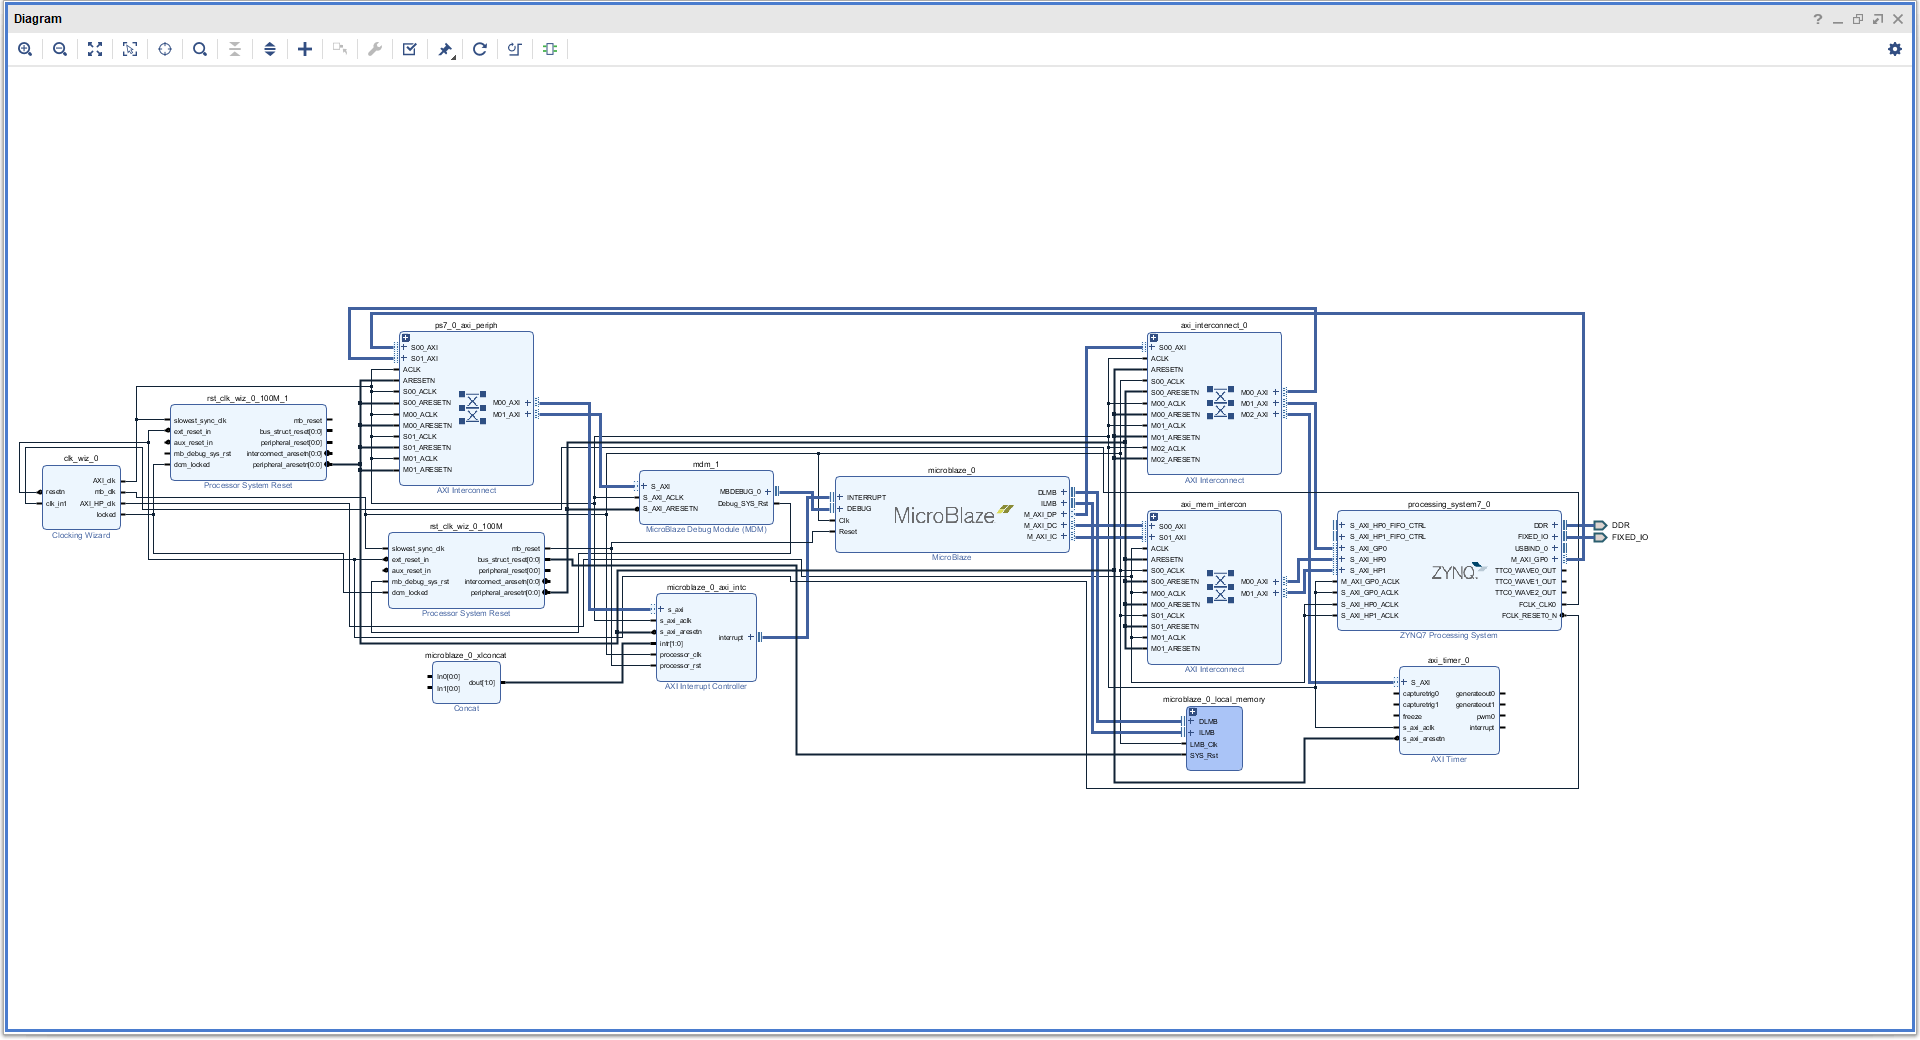
\includegraphics[width=\linewidth]{im/mb1.png}	
	\caption{Exemple de design pour le Multi CPU}
	\label{fig-mb}
\end{figure}
Ce design permet de faire tourner un programme sur le FPGA et sur le microblaze.


Maintenant que le microblaze est rajouté, il peut être intéréssant de pouvoir lui passer des donnée. Le microblaze est déja connecté à la RAM du ZYNQ donc en théorie il peut déja recevoir et envoyé des donnés.\\
On peut déja les faire s'exécuter tout les 2 depuis la RAM du ZYNQ (cela permet d'agrandir le heap et le stack pour éviter les dépassement).
\begin{figure}[H]
	\centering
		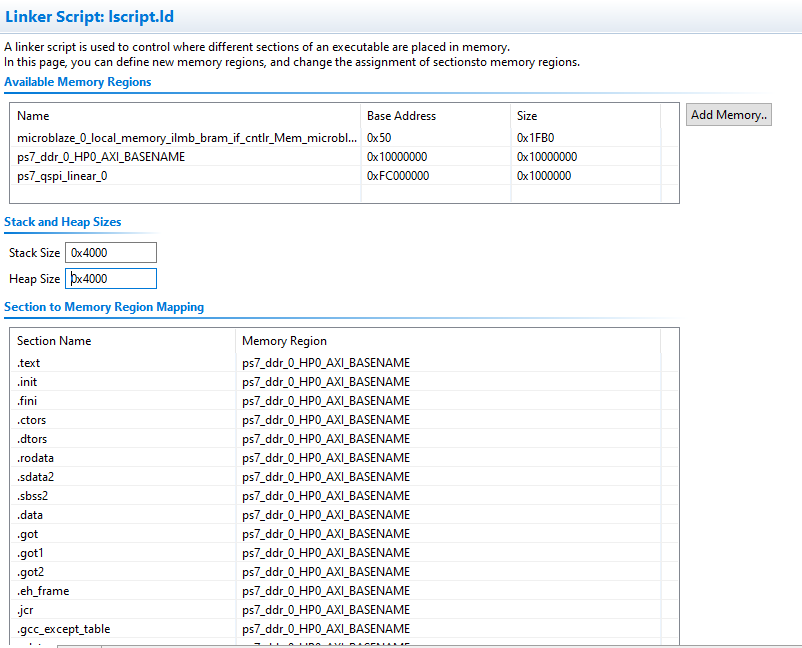
\includegraphics[width=\linewidth]{im/mb2.png}	
	\caption{Linker script du microblaze : exécution depuis la DDR et stack et heap étendus}
	\label{fig-link}
\end{figure}

Une des chose que l'on voudrait pouvoir faire c'est passé une grande quantité de donnée et des instruction au microblaze.\\
Du fait qu'il a accès à la RAM du \textit{Zynq} il faudrait juste pouvoir lui envoyer des instructions. Si possible dans un emplacement fixe de la mémoire.
\subsubsection{Utilisation de la BRAM}
Pour passer des instruction du \textit{Zynq} au \textit{microblaze}, On décide d'utiliser les BRAM.

On crée ainsi un block design qui a en plus du lien avec la DDR du \textit{Zynq}, a aussi des BRAMs. A l'intérieur de celles-ci, on pourra placer des adresses pour les données et des instructions sur ce qu'il faudra en faire.

\begin{figure}[H]
	\centering
		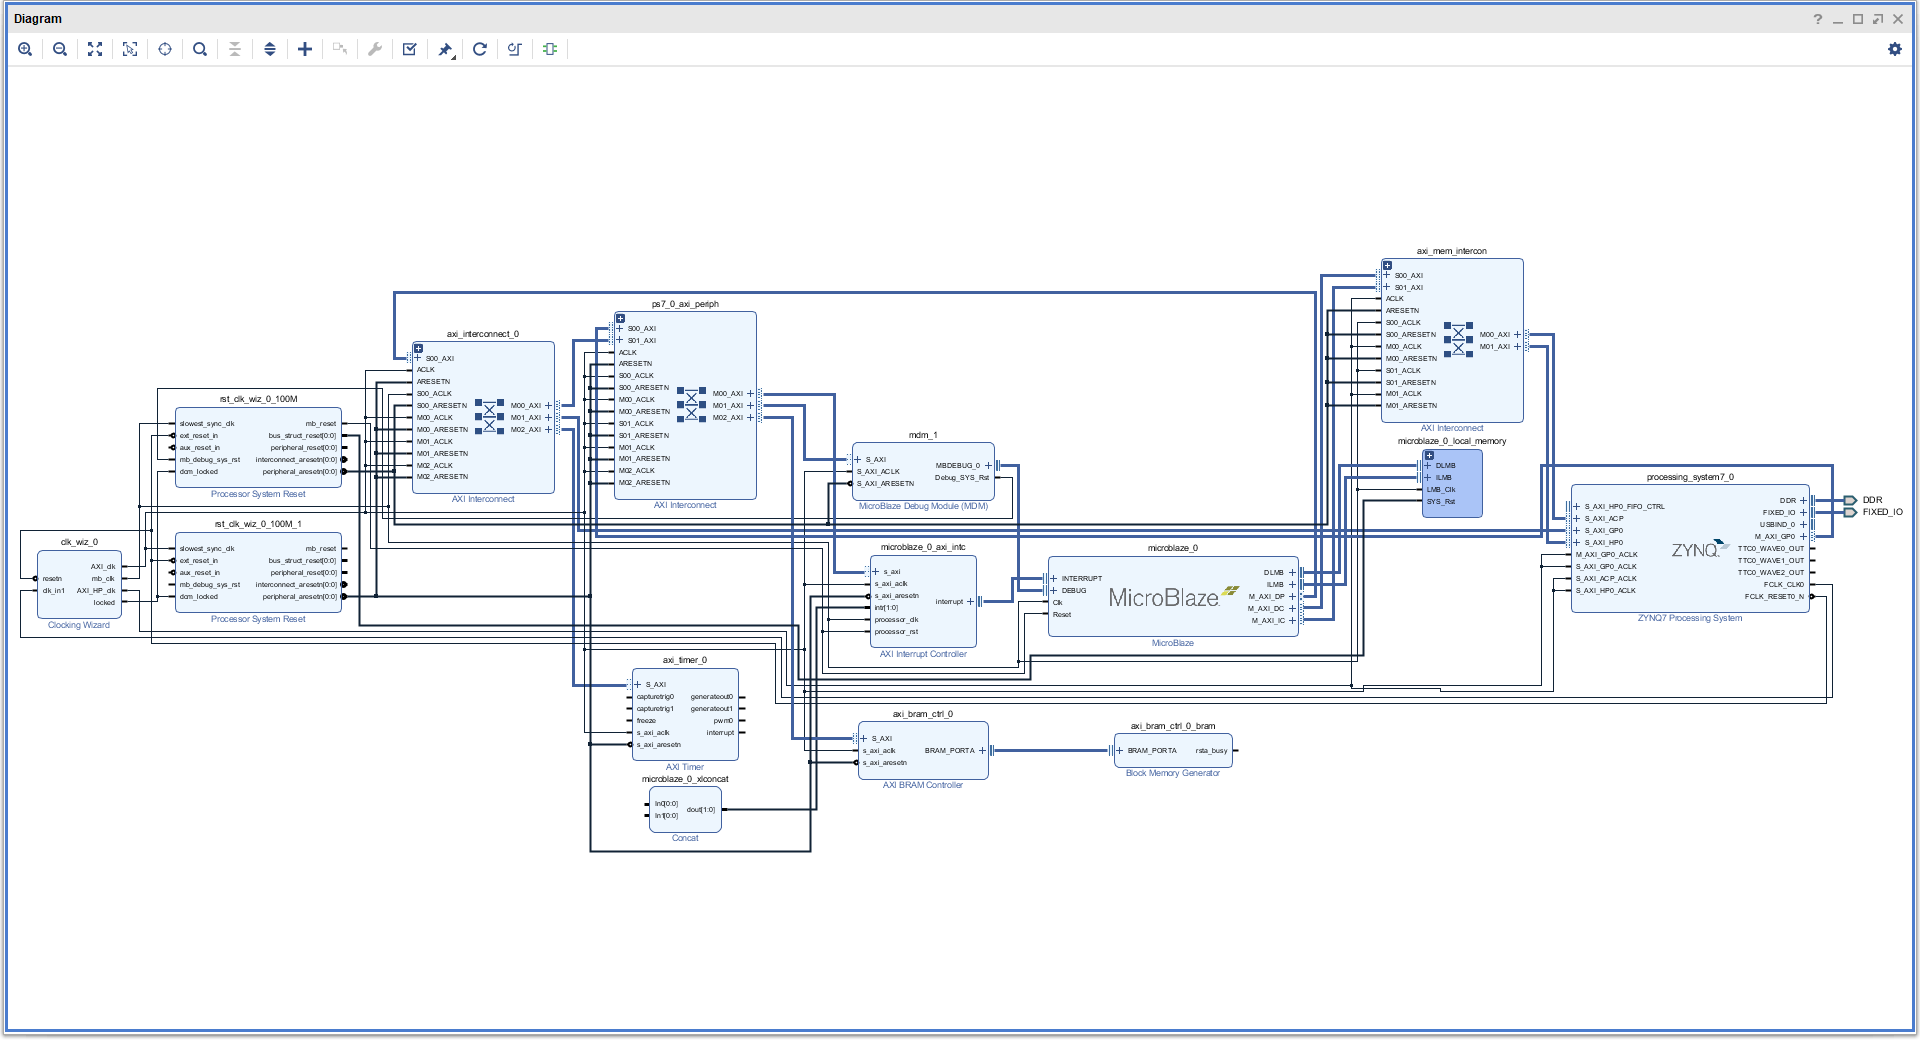
\includegraphics[width=\linewidth]{im/bram1.png}	
	\caption{Block design pour tester la BRAM :}
	\label{fig-bram1}
\end{figure}


\subsubsection{Passage de données vers un microblaze}
Une fois cela fait la BRAM on a développé 2 applications : une pour le \textit{Zynq} et une pour le \textit{microblaze}.



\begin{figure}[H]
\begin{multicols}{2}
		\begin{lstlisting}[language=C]
		
int main()
{
	XTime Start_Time, End_Time;

    init_platform();

    print("Zynq:Hello World\n\r");
    XTime_GetTime((XTime *) &Start_Time);
    char * test =(char*)XPAR_AXI_BRAM_CTRL_0_S_AXI_BASEADDR;

    memcpy(test,"un message\n",20);

    while(1){
    	 XTime_GetTime((XTime *) &End_Time);
    	 sprintf(test,"message à %lli",(End_Time - Start_Time));
    	sleep(1);
    }
	\end{lstlisting}	
	 \bigskip
			\begin{lstlisting}[language=C]
int main()
{
	char* test=(char*)XPAR_AXI_BRAM_CTRL_0_S_AXI_BASEADDR;
    init_platform();

    print("micro:Hello World 2\n\r");
	sleep(10);
    
    
    
    while(1){
    	printf("micro:%s\n",test);
    	sleep(1);
    }
}

	\end{lstlisting}	
\end{multicols}		
	\caption{Code du microblaze(droite) et du zynq(gauche) pour l'envoie et la réception de message}
	\label{fig-hls}
\end{figure}
On peut ainsi facilement passer des adresses du Zynq au microblaze grace à la BRAM.
\begin{figure}[H]
	\centering
		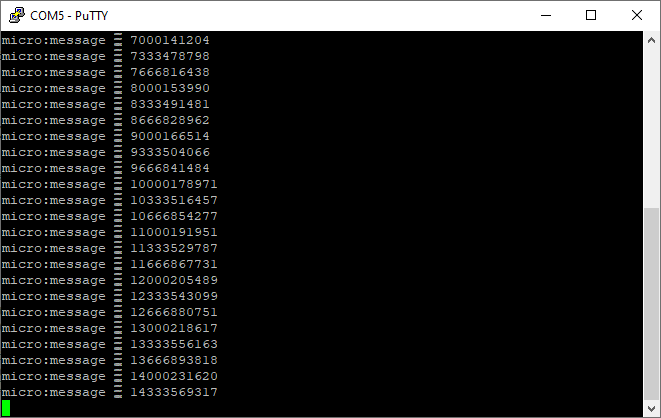
\includegraphics[width=\linewidth]{im/bram2.png}	
	\caption{Démonstration de la BRAM : le microblaze affiche un message envoyé depuis le Zynq}
	\label{fig-bram2}
\end{figure}

La finalité de ce design a été de permettre à l'équipe logicielle de testé leur programme sur la carte.
\subsection{IP HLS}
Dès que les première IP HLS ont été finalisés, il a été question de les intégrées dans un design.\\
Un design a été conçu pour tester.
\subsubsection{Concept}
Pour accélérer, les programmes que l'on fait tourner sur les \textit{Zynq}, la partie HLS à réaliser des accélérateur à l'aide des outils \textit{Xilinx}. Ces accélérateurs ce présente comme des IP que l'on peut rajouter dans un block design.

Il faudra envoyer des donnés à ces IP pour quelle fasse les calculs à la place du \textit{Zynq} : Beaucoup plus rapidement.\\

Ces IP sont commandés par le \textit{Zynq} qui leur donne également des emplacement mémoire comme paramètre.\
Elles dispose d'accès directe à la mémoire DDR du \textit{Zynq} pour pouvoir charger localement les donné et ranger les résultats.\\

\subsubsection{Implémentation et clocking}
Une fois les IP mis dans un repos communs et que ce repertoire est signaler à \textit{ Vivado} comme contenant des IPs, On peut les utiiliser dans un block design classique.
\subsubsubsection{Relier les IP aux Zynq}
Les IPs HLS se presente comme suivant:
\begin{figure}[H]
	\centering
		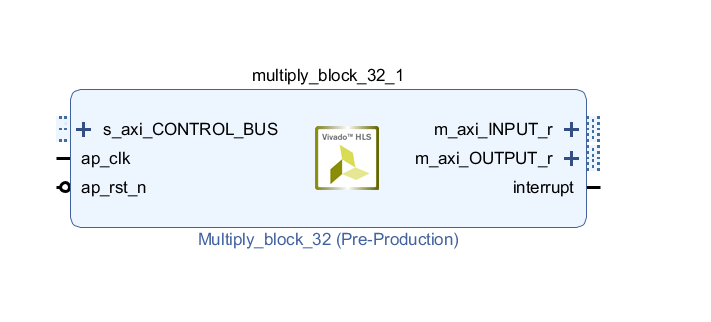
\includegraphics[width=\linewidth]{im/ip1.png}	
	\caption{Exemple d'IP on voit les différent port}
	\label{fig-ip1}
\end{figure}

Elles ont 6 ports: \begin{itemize}
\item[•]Un Port Slave AXILite appelé \lstinline[language=bash]{CONTROL_BUS} qui sert a commandé l'IP.
\item[•]2 Port Master AXI appelé \lstinline[language=bash]{INPUT} et \lstinline[language=bash]{OUTPUT} qui servent à l'IP pour accédé à des données en mémoire.
\item[•] Des port \lstinline[language=bash]{clk} et \lstinline[language=bash]{rst} qui permettent à l'IP d'avoir une clock indépendante (on utilisera cela pour avoir de meilleur performance)
\item[•]Un port \lstinline[language=bash]{interrupt} qui n'as pas été utilisé mais pourrait être utilisé avec un microblaze pour déclenché une interruption dès que l'IP fini.

\end{itemize}

On relis cette IP au Zynq de la manière suivante:\begin{itemize}
\item[•]Les ports \lstinline[language=bash]{INPUT} et \lstinline[language=bash]{OUTPUT} sont relié au Slave ACP du ZYNQ pour pouvoir accédé à ces mémoire et avoir la cohérence des caches.(figure \ref{fig-acp}).
\item[•] On relis les port \lstinline[language=bash]{CONTROL_BUS} au Master GP du Zynq pour pouvoir envoyer des commandes (les commandes étant moins critique ne pas passer par les interface rapide ne pose pas trop de problème)
\end{itemize}


\begin{figure}[H]
	\centering
		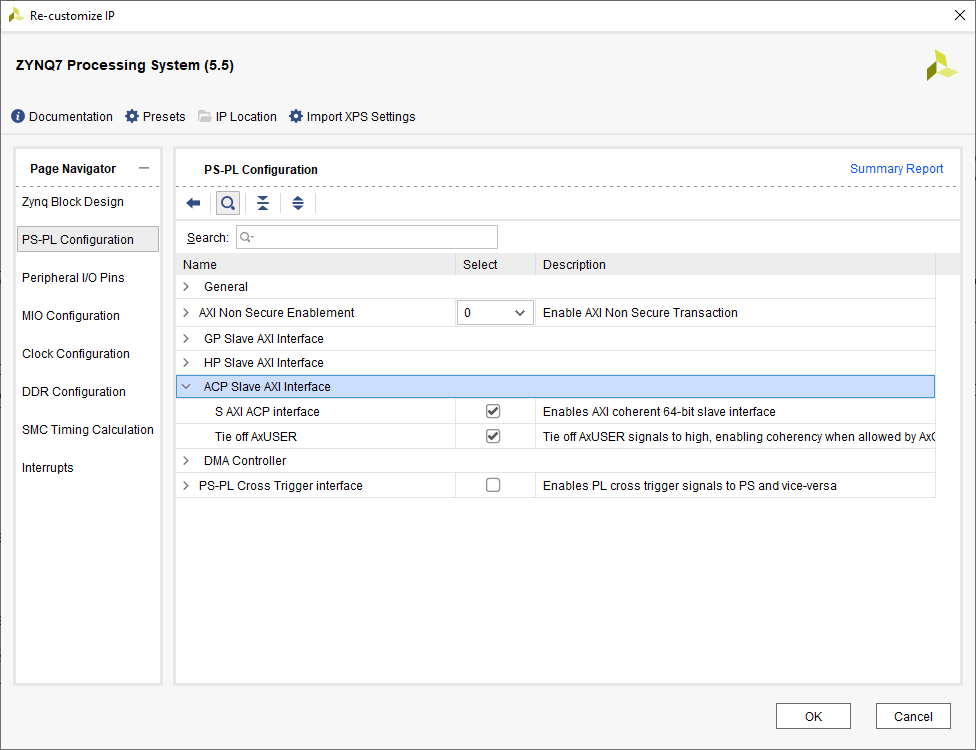
\includegraphics[width=\linewidth]{im/ip2.png}	
	\caption{Paramètre du Zynq: ce qu'il faut cocher pour avoir l'interface ACP et la cohérence des caches}
	\label{fig-acp}
\end{figure}

\begin{figure}[H]
	\centering
		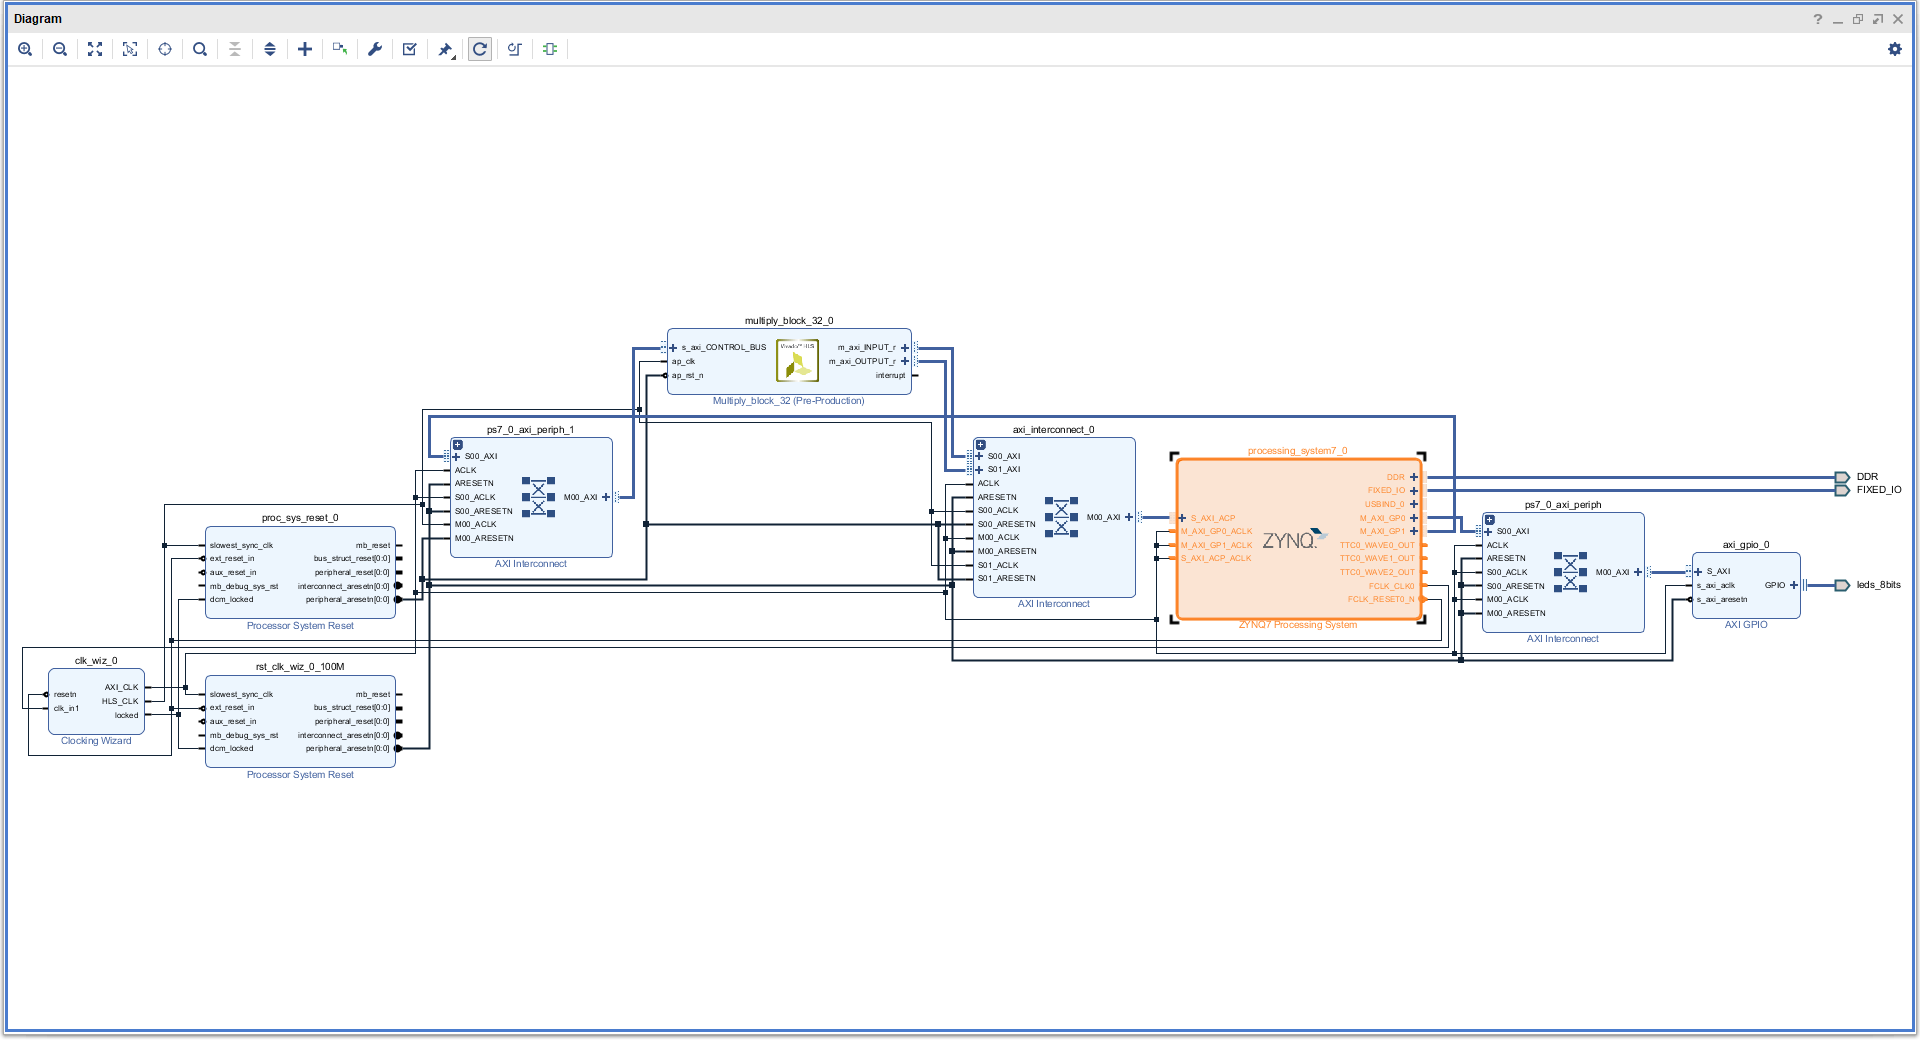
\includegraphics[width=\linewidth]{im/ip3.png}	
	\caption{Exemple de design pour l'IP multiply\_block\_32}
	\label{fig-ip}
\end{figure}
On a fait en sorte dans les bock design que les clock des IP et la clock du HLS soit indépendantes. Cela permettra de tiré le plus de performance des IP plus tard.


\subsubsubsection{Fonction pour le SDK}
A partir de là, après synthèse placement et routage du design, on dispose d'un entête spécial par exemple:
\begin{lstlisting}[language=C]
#include "xmultiply_block_64.h"
\end{lstlisting}
qui va permettre d'interagir simplement avec une IPS HLS.\\

Ainsi le code suivant contient 2 fonctions qui permettent d'initialiser une IP HLS(ici \textit{mul64}) et de l'utiliser pour faire un calcul.
\begin{lstlisting}[language=C]
//fonction d'initilisation de L'IP
void init_multiply_block_ip(XMultiply_block_64* mb,XMultiply_block_64_Config* mb_c){
	int status=XMultiply_block_64_CfgInitialize(mb,mb_c);
	XMultiply_block_64_DisableAutoRestart(mb);
	XMultiply_block_64_InterruptGlobalDisable(mb);
	XMultiply_block_64_InterruptDisable(mb, 1);
	if(status!=XST_SUCCESS){
		printf("Multiply Block: init_failed \r\n");
	}
	printf("idle=%lx,ready=%lx,done=%lx\n",XMultiply_block_64_IsIdle(mb),XMultiply_block_64_IsReady(mb),XMultiply_block_64_IsDone(mb));
	printf("succes\n");
}

//fonction de lancement du calcul sur l'IP
void multiply_block_hw_call(XMultiply_block_64* mb_p,float* mA, float* mB, float* result){

	//on charge les adresse des données et les sorties
	XMultiply_block_64_Set_in_mA(mb_p, (u32)mA);
	XMultiply_block_64_Set_in_mB(mb_p, (u32)mB);
	XMultiply_block_64_Set_out_mC(mb_p, (u32)result);

	//on attend d'être prêts.
	while(!XMultiply_block_64_IsReady(mb_p));
	
	//on lance
	XMultiply_block_64_Start(mb_p);
	
	//on attend d'avoir fini	
	while(!XMultiply_block_64_IsDone(mb_p)){
		
	}
	//les résultat sont déja rangé donc on a fini.
	return;

}

\end{lstlisting}
Grâce à l'utilisation des interfaces ACP et du fait qu'on ait activé le "\textit{tie off AxUser}", nous n'avons pas besoin de vider le cache puisque la cohérence est maintenu à travers l'AXI et malgré les modification des données faite par l'IP.


\subsubsubsection{Optimisation des clock avec les Timings}
On peut maintenant chercher à avoir le plus de performances possible avec nos IPs. Pour cela on va utiliser le fait qu'elle aient des clock indépendantes de celle de l'AXI. On peut ainsi changer leur fréquence séparément du reste du système.\\

Grâce au \textit{timing report} on peut connaitre après implémentation quelle est la marge que l'on a par rapport au temps critique fixé par la clock. On peut ainis corriger cette clock itérativement pour aller jusqu'au moment ou l'on n'a plus aucune marge.

On a put par exemple monter la clock de l'IP \textit{mul64} de 100 à 130 MHZ.

\begin{figure}[H]
	\centering
		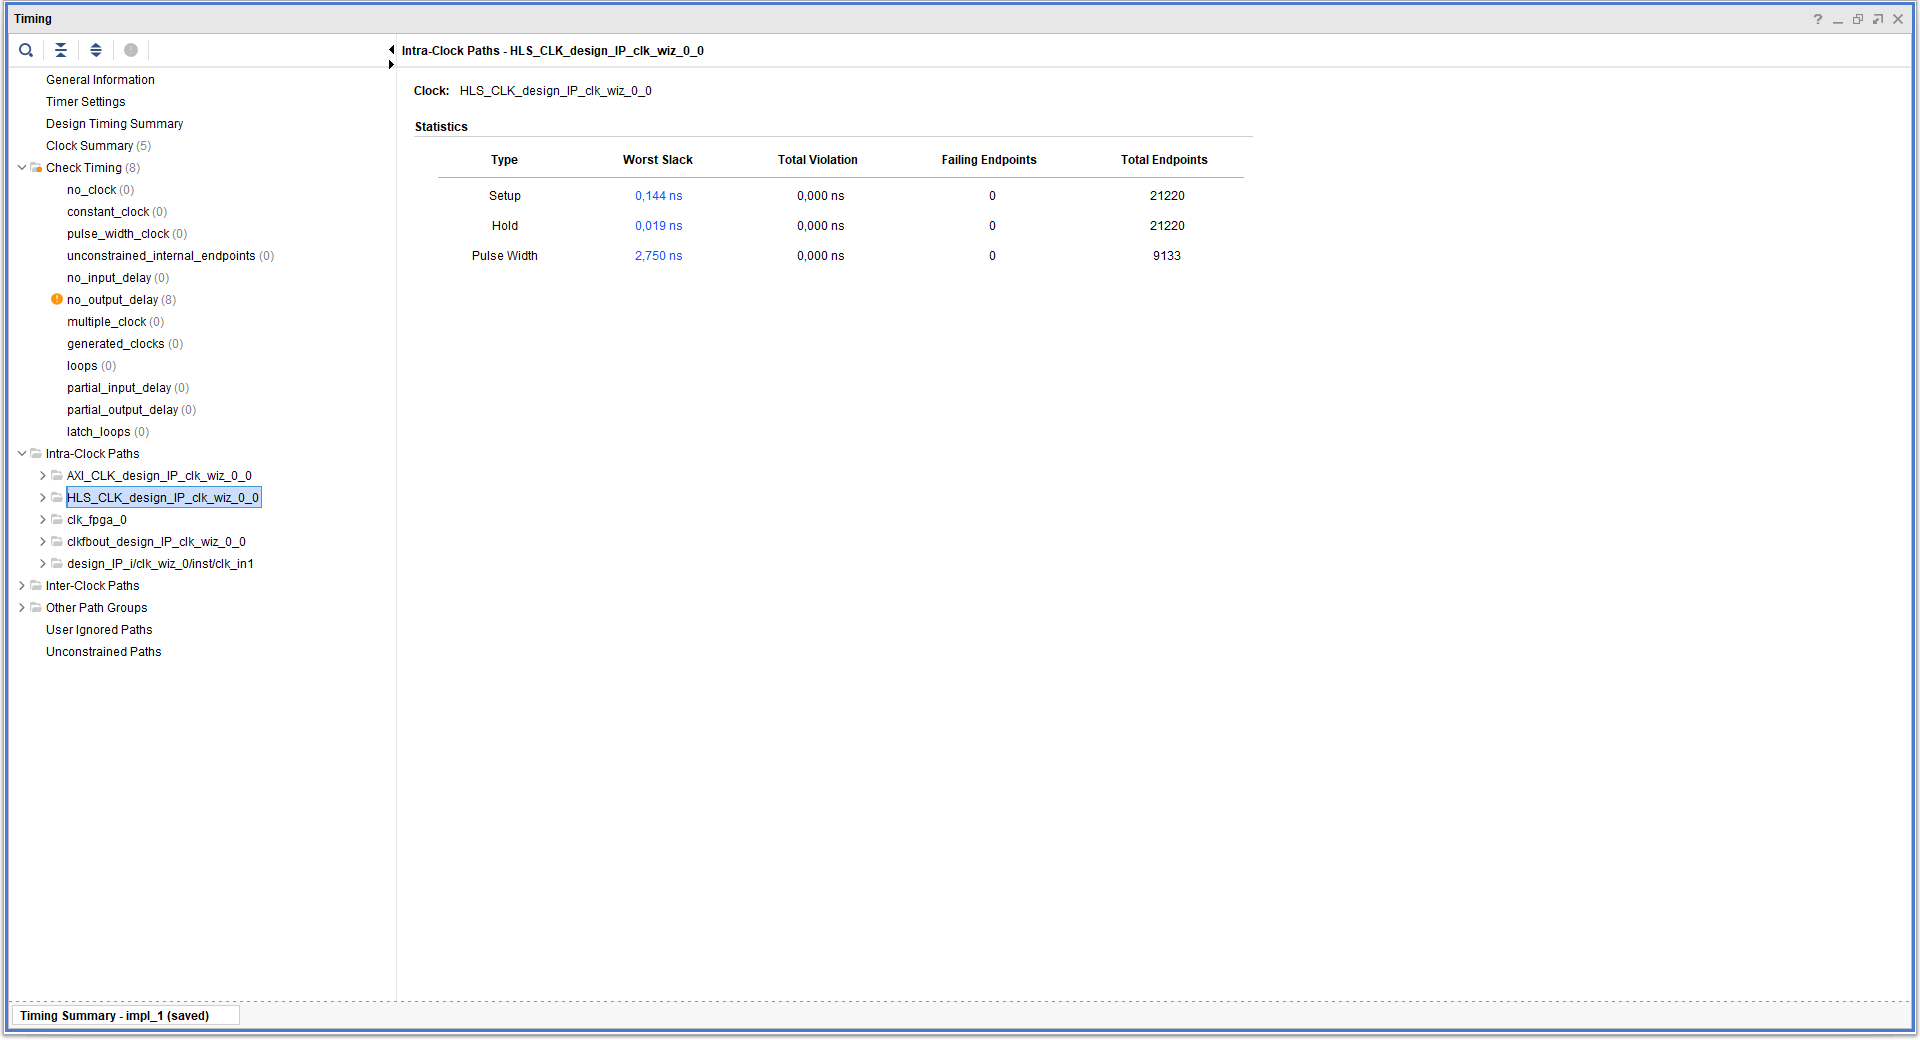
\includegraphics[width=\linewidth]{im/timing.png}	
	\caption{Ecran du timing report permettant de connaitre le clock skew}
	\label{fig-clk}
\end{figure}

\subsubsection{Performances}
En mesurant le temps grâce au timer du \textit{Zynq} on peut évaluer les performance des IPs.\\
Les IPs évalués sont: \begin{itemize}
\item[•]Block matrix multiplication 32 par 32(\textit{mul32}) et 64 par 64(\textit{mul64})
\item[•]Le coefficient de Pearson (\textit{pearson})
\item[•]L'algorithme kmeans (\textit{kmeans}
\end{itemize}
\bigskip
On compare ainsi les temps Software, Hardware et Hardware avec clock amélioré:\\
\bigskip
\begin{tabular}{|c|c|c|c|c|}

\hline
\scriptsize exemple d'IP & \scriptsize temps HW ($\mu s$) @100MHZ &\scriptsize temps SW ($\mu s$) &\scriptsize fréquence amélioré&\scriptsize temps HW amélioré($\mu s$) \\
\hline
mul64 & 10280.17417 & 26132.32432 & 130 MHZ & 7042.11712 useconds\\
mul32&2411.54655  & 3281.83483& 125MHZ & 1809.89489\\
pearson&  &5.25826 &115 MHZ &21.19820\\
kmeans&1297.41742 & 1120841.13814 &120MHZ &1082.07808\\
\hline
\end{tabular}\\
\bigskip
On a aussi essayé de serrer encore plus les timing en jouant sur la Clock des AXI et sur l'algorithme de placement (Haute performance).\\
Avec les réglages suivant : \begin{itemize}
\item[•]AXI\_CLK=180MHZ
\item[•]HLS\_CLK=131MHZ
\end{itemize}
On a un temps de 6215.74174 $\mu s$ soit plus de 4 fois moins de temps que la version SW classique.


\subsection{Amélioration et future design}
Il s'agirait ensuite de construire un design utilisant et les IP et le \textit{microblaze} pour pouvoir, par exemple utiliser l'IP HLS de block matrix multiplication. Pour faire des multiplication de matrice plus grande en utilisant plusieurs fois l'IP sans avoir besoin de monopoliser le \textit{Zynq}, utilisant ainsi les interruption sur le \textit{microblaze.}

%exemple d'achitecture en cours de developemnt mais qui n'as pas put être fini.

\end{document}